\newcommand\addrow[2]{#1 &#2\\ }

\newcommand\addheading[2]{#1 &#2\\ \hline}
\newcommand\tabularhead{\begin{tabular}{lp{11cm}}
\hline
}
\newcommand\addmulrow[2]{ \begin{minipage}[t][][t]{2.5cm}#1\end{minipage}% 
   &\begin{minipage}[t][][t]{11cm}
    \begin{enumerate} #2   \end{enumerate}
    \end{minipage}\\ }

\newenvironment{usecase}{\tabularhead}
{\hline\end{tabular}}

\iffalse
\begin{usecase}
  \addheading{Actor}{System user} 
  \addrow{Precondición}{The system, shows, in the form part of an object type, the number   indication.}
  \addrow{Postcondición}{A disconnected number indicating the type of `other constructed object'.}
  \addmulrow{Escenario principal}{\item User selects \ldots
                                   \item System demands \ldots}
\end{usecase}
\fi


En la especificación se concretaran todos los artefactos, donde se desglosara conceputalmente las características, elementos y servicios necesarios para desarrollar el proyecto.

\subsection{Casos de uso}
Los casos de uso explican los pasos o actividades que los actores tendrán que realizar para llevar a acabo algún proceso, los actores son los que hemos visto en el análisis de requisitos. A continuación se desglosan los casos de uso divididos por actor.

\subsubsection{Usuario final}
El siguiente diagrama explica de forma visual las interacciones del usuario final con el sistema, a continuación se encuentras las tablas que detallan cada caso de uso.

\begin{figure}[ht!]
\center
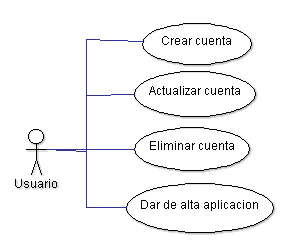
\includegraphics[scale=1.0]{diagramas/usecase_user1.png}
\end{figure}

\begin{usecase}
\textbf{Crear cuenta}\\
  \addheading{Actor}{Usuario final} 
  \addrow{Precondición}{-}
  \addrow{Postcondición}{El usuario dispone de una cuenta con la que acceder al sistema.}
  \addmulrow{Escenario principal}{
	  	\item El usuario introduce los datos requeridos por el sistema y los confirma.
		\item El sistema da de alta al usuario
	}
  \addmulrow{Escenario\\ alternativo}{
	  	\item El usuario introduce los datos requeridos por el sistema y los confirma.
		\item El sistema avisa al usuario que los datos introducidos no son correctos.
		\item Se vuelve a ejecutar el caso de uso crear cuenta.
	}
\end{usecase}
\\
\begin{usecase}
\textbf{Actualizar cuenta}\\
  \addheading{Actor}{Usuario final} 
  \addrow{Precondición}{El usuario esta dado de alta en el sistema}
  \addrow{Postcondición}{El usuario a actualizado sus datos de usuario en el sistema.}
  \addmulrow{Escenario principal}{
	  	\item El usuario introduce los datos requeridos por el sistema y los confirma.
		\item El sistema actualiza los datos del usuario
	}
  \addmulrow{Escenario\\ alternativo}{
	  	\item El usuario introduce los datos requeridos por el sistema y los confirma.
		\item El sistema avisa al usuario que los datos introducidos no son correctos.
		\item Se vuelve a ejecutar el caso de uso actualizar cuenta.
	}
\end{usecase}
\\
\begin{usecase}
\textbf{Eliminar cuenta}\\
  \addheading{Actor}{Usuario final} 
  \addrow{Precondición}{El usuario esta dado de alta en el sistema}
  \addrow{Postcondición}{El usuario es dado de baja del sistema.}
  \addmulrow{Escenario principal}{
	  	\item El usuario indica al sistema que se quiere dar de baja.
		\item El sistema da de baja al usuario del sistema.
	}
\end{usecase}
\\
\begin{usecase}
\textbf{Dar de alta aplicación}\\
  \addheading{Actor}{Usuario final} 
  \addrow{Precondición}{El usuario esta dado en alta en el sistema}
  \addrow{Postcondición}{El usuario proporciona los datos necesarios para dar de alta la aplicación.}
  \addmulrow{Escenario principal}{
	  	\item El usuario introduce los datos requeridos por el sistema y los confirma.
		\item El sistema da de alta la nueva aplicación.
	}
  \addmulrow{Escenario\\ alternativo}{
	  	\item El usuario introduce los datos requeridos por el sistema y los confirma.
		\item El sistema avisa al usuario que los datos introducidos no son correctos.
		\item Se vuelve a ejecutar el caso de uso dar de alta aplicación.
	}
\end{usecase}
\newpage

\begin{figure}[ht!]
\center
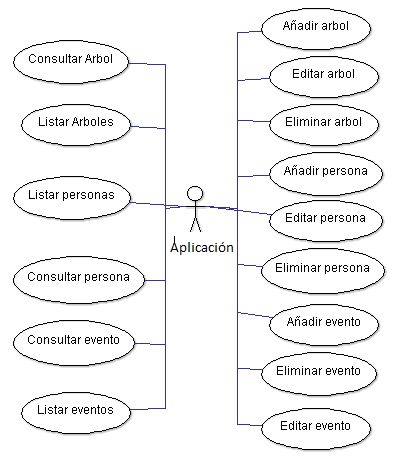
\includegraphics[scale=1.0]{diagramas/usecase_aplication.png}
\end{figure}
\begin{figure}[ht!]
\center
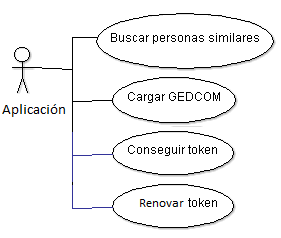
\includegraphics[scale=1.0]{diagramas/usecase_aplication2.png}
\end{figure}

\begin{usecase}
\textbf{Conseguir token}\\
  \addheading{Actor}{Aplicación} 
  \addrow{Precondición}{La aplicación esta dada en alta en el sistema}
  \addrow{Postcondición}{El sistema devuelve un token que valida un usuario contra el sistema.}
  \addmulrow{Escenario principal}{
	  	\item La aplicación pide un token al sistema dando sus credenciales y las de un usuario.
		\item El sistema retorna a la aplicación un token que contiene la información para validad un usuario a través suyo.
	}
  \addmulrow{Escenario\\ alternativo}{
	  	\item La aplicación pide un token al sistema dando sus credenciales y las de un usuario.
		\item Retorna un mensaje de error indicando que credenciales no son correctos.
		\item Se vuelve a ejecutar el caso de uso conseguir token.
	}
\end{usecase}
\newpage
\begin{usecase}
\textbf{Renovar token}\\
  \addheading{Actor}{Aplicación} 
  \addrow{Precondición}{La aplicación esta dada en alta en el sistema}
  \addrow{Postcondición}{El sistema devuelve un token que valida un usuario contra el sistema.}
  \addmulrow{Escenario principal}{
	  	\item La aplicación pide la renovación de un token al sistema dando sus credenciales y las credenciales que permiten renovar un token concreto.
		\item El sistema retorna a la aplicación un token que contiene la información para validad un usuario a través suyo.
	}
  \addmulrow{Escenario\\ alternativo}{
	  	\item La aplicación pide la renovación de un token al sistema dando sus credenciales y las credenciales que permiten renovar un token concreto.
		\item Retorna un mensaje de error indicando que credenciales no son correctos.
		\item Se vuelve a ejecutar el caso de uso renovar token.
	}
\end{usecase}
\newpage
\begin{usecase}
\textbf{Añadir árbol}\\
  \addheading{Actor}{Aplicación} 
  \addrow{Precondición}{La aplicación esta dada en alta en el sistema}
  \addrow{Postcondición}{El sistema añade el árbol con los datos proporcionados.}
  \addmulrow{Escenario principal}{
	  	\item La aplicación envía una petición al servidor con los datos necesarios para dar de alta un árbol y el token de un usuario.
		\item El sistema confirma la creación del árbol a la aplicación.
	}
  \addmulrow{Escenario\\ alternativo}{
	  	\item La aplicación envía una petición al sistema con los datos necesarios para dar de alta un árbol y el token de un usuario.
		\item Retorna un mensaje de error indicando que el token no es valido.
		\item Se va a ejecutar el caso de uso conseguir token.
	}
  \addmulrow{Escenario\\ alternativo}{
	  	\item La aplicación envía una petición al servidor con los datos necesarios para dar de alta un árbol y el token de un usuario.
		\item Retorna un mensaje de error indicando que el token esta caducado.
		\item La aplicación ejecuta el caso de uso renovar token.
	}
  \addmulrow{Escenario\\ alternativo}{
 	\item La aplicación envía una petición al servidor con los datos necesarios para dar de alta un árbol y el token de un usuario.
 	\item Retorna un mensaje de error indicando que el árbol no es valido.
 }
\end{usecase}
\newpage
\begin{usecase}
\textbf{Editar árbol}\\
  \addheading{Actor}{Aplicación} 
  \addrow{Precondición}{La aplicación esta dada en alta en el sistema}
  \addrow{Postcondición}{El sistema actualiza el árbol con los datos proporcionados.}
  \addmulrow{Escenario principal}{
	  	\item La aplicación envía una petición al servidor con los datos necesarios para actualizar los datos de un árbol y el token de un usuario.
		\item El sistema confirma que los datos del árbol han modificado a la aplicación.
	}
  \addmulrow{Escenario\\ alternativo}{
	  	\item La aplicación envía una petición al sistema con los datos necesarios para actualizar los datos de un árbol y el token de un usuario.
		\item Retorna un mensaje de error indicando que el token no es valido.
		\item Se vuelve a ejecutar el caso de uso conseguir token.
	}
  \addmulrow{Escenario\\ alternativo}{
	  	\item La aplicación envía una petición al sistema con los datos necesarios para actualizar los datos de un árbol y el token de un usuario.
		\item Retorna un mensaje de error indicando que el token esta caducado.
		\item La aplicación ejecuta el caso de uso renovar token.
	}
	\addmulrow{Escenario\\ alternativo}{
		\item La aplicación envía una petición al sistema con los datos necesarios para actualizar los datos de un árbol y el token de un usuario.
		\item Retorna un mensaje de error indicando que el árbol no existe.
	}
	\addmulrow{Escenario\\ alternativo}{
		\item La aplicación envía una petición al sistema con los datos necesarios para actualizar los datos de un árbol y el token de un usuario.
		\item Retorna un mensaje de error indicando que el árbol no es valido.
	}
\end{usecase}
\newpage
\begin{usecase}
\textbf{Eliminar árbol}\\
  \addheading{Actor}{Aplicación} 
  \addrow{Precondición}{La aplicación esta dada en alta en el sistema}
  \addrow{Postcondición}{El sistema elimina el árbol con los datos proporcionados.}
  \addmulrow{Escenario principal}{
	  	\item La aplicación envía una petición al sistema con los datos necesarios para eliminar un árbol y el token de un usuario.
		\item El sistema confirma el árbol ha sido eliminado a la aplicación.
	}
  \addmulrow{Escenario\\ alternativo}{
	  	\item La aplicación envía una petición al sistema con los datos necesarios para eliminar un árbol y el token de un usuario.
		\item Retorna un mensaje de error indicando que el token no es valido.
		\item Se vuelve a ejecutar el caso de uso conseguir token.
	}
  \addmulrow{Escenario\\ alternativo}{
	  		  	\item La aplicación envía una petición al sistema con los datos necesarios para eliminar un árbol y el token de un usuario.
		\item Retorna un mensaje de error indicando que el token esta caducado.
		\item La aplicación ejecuta el caso de uso renovar token.
	}
\end{usecase}
\newpage
\begin{usecase}
\textbf{Consultar árbol}\\
  \addheading{Actor}{Aplicación} 
  \addrow{Precondición}{La aplicación esta dada en alta en el sistema}
  \addrow{Postcondición}{El sistema retorna la información de árbol consultado.}
  \addmulrow{Escenario principal}{
	  	\item La aplicación envía una petición al sistema con los datos necesarios para consultar un árbol y el token de un usuario.
		\item El sistema retorna los datos del árbol consultado
	}
  \addmulrow{Escenario\\ alternativo}{
	  	\item La aplicación envía una petición al sistema con los datos necesarios para consultar un árbol y el token de un usuario.
		\item Retorna un mensaje de error indicando que el token no es valido.
		\item Se ejecuta el caso de uso conseguir token.
	}
  \addmulrow{Escenario\\ alternativo}{
	  	\item La aplicación envía una petición al sistema con los datos necesarios para consultar un árbol y el token de un usuario.
		\item Retorna un mensaje de error indicando que el token esta caducado.
		\item La aplicación ejecuta el caso de uso renovar token.
	}
\end{usecase}
\newpage
\begin{usecase}
\textbf{Cargar árbol}\\
  \addheading{Actor}{Aplicación} 
  \addrow{Precondición}{La aplicación esta dada en alta en el sistema}
  \addrow{Postcondición}{El sistema almacena el árbol.}
  \addmulrow{Escenario principal}{
	  	\item La aplicación envía una petición al sistema con los datos necesarios para cargar un árbol y el token de un usuario.
		\item El sistema carga todos los datos del árbol enviado por la aplicación.
		\item El sistema confirma la operación
	}
  \addmulrow{Escenario\\ alternativo}{
	  	\item La aplicación envía una petición al sistema con los datos necesarios para cargar un árbol y el token de un usuario.
		\item Retorna un mensaje de error indicando que el token no es valido.
		\item Se ejecuta el caso de uso conseguir token.
	}
  \addmulrow{Escenario\\ alternativo}{
	  	\item La aplicación envía una petición al sistema con los datos necesarios para consultar un árbol y el token de un usuario.
		\item Retorna un mensaje de error indicando que el token esta caducado.
		\item La aplicación ejecuta el caso de uso renovar token.
	}
\addmulrow{Escenario\\ alternativo}{
	  	\item La aplicación envía una petición al sistema con los datos necesarios para cargar un árbol y el token de un usuario.
		\item Retorna un mensaje de error indicando que el los datos del árbol a cargar no son validos.
	}
\end{usecase}
\newpage
\begin{usecase}
\textbf{Buscar personas similares}\\
  \addheading{Actor}{Aplicación} 
  \addrow{Precondición}{La aplicación esta dada de alta en el sistema}
  \addrow{Postcondición}{El sistema confirma que se ha aceptado la petición y crea conexiones entre los usuarios similares.}
  \addmulrow{Escenario principal}{
	  	\item La aplicación envía una petición al sistema con los datos que identifican a una persona y el token de un usuario.
		\item El sistema crea las conexiones entre los usuarios similares.
		\item El sistema confirma la operación al usuario
		\item El sistema confirma por correo electrónico que la operación ha finalizado y el estado.
	}
  \addmulrow{Escenario\\ alternativo}{
	  		\item La aplicación envía una petición al sistema con los datos que identifican a una persona y el token de un usuario.
		\item Retorna un mensaje de error indicando que el token no es valido.
		\item Se ejecuta el caso de uso conseguir token.
	}
  \addmulrow{Escenario\\ alternativo}{
	  		\item La aplicación envía una petición al sistema con los datos que identifican a una persona y el token de un usuario.
		\item Retorna un mensaje de error indicando que el token esta caducado.
		\item La aplicación ejecuta el caso de uso renovar token.
	}
\addmulrow{Escenario\\ alternativo}{
	  		\item La aplicación envía una petición al sistema con los datos que identifican a una persona y el token de un usuario.
		\item Retorna un mensaje de error indicando que el los datos del de la persona no son validos.
	}
\end{usecase}

*Los casos de uso referentes a las operaciones CRUD de los otros objetos del modelo funcionan con la mima lógica que las operaciones CRUD del árbol.\\
Por lo tanto no se especifican.

\newpage
\subsection{Modelo conceptual de datos}
\label{sec:smodelo_conceptual_datos}
El modelo conceptual de datos, es la representación de los conceptos significativos en el dominio del problema, es decir, son las principales entidades que forman el sistema a partir de ahora estas entidad las llamaremos clases.
El siguiente diagrama explica como se relacionan las clases de nuestro modelo de datos entre ellos en UML (Unified Modeling Language).
\begin{figure}[ht!]
\center
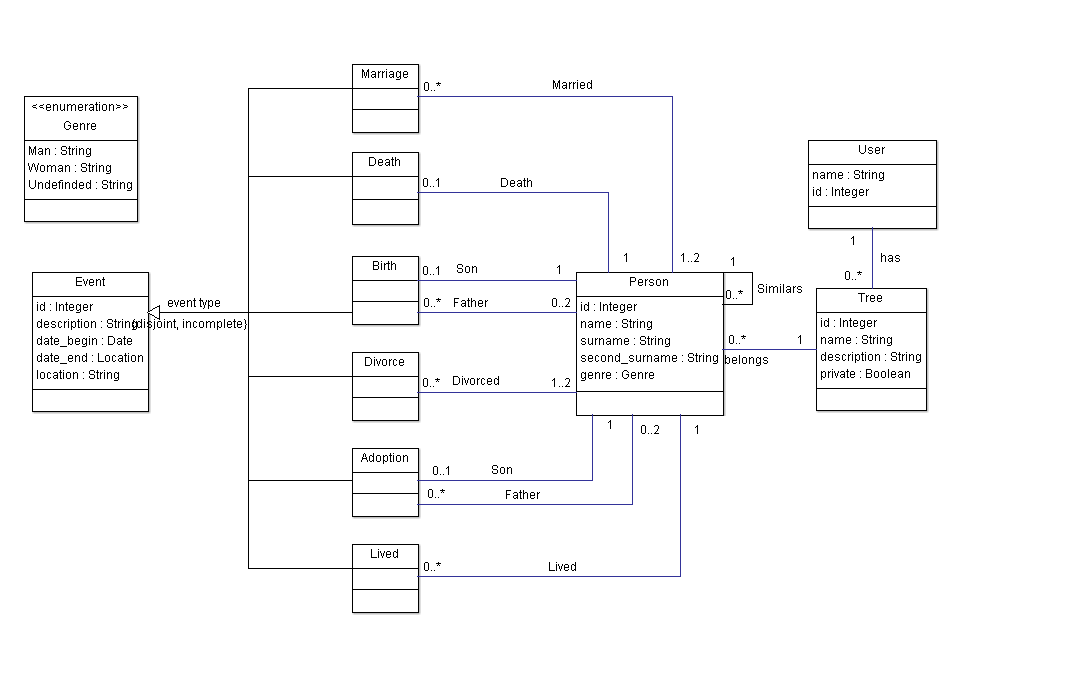
\includegraphics[width=\textwidth,height=\textheight,keepaspectratio]{diagramas/datamodel.png}
\caption{Diagrama del modelo conceptual de datos}
\label{fig:data_model}
\end{figure}

A continuación se explica que representa cada clase de nuestro modelo.
\begin{description}
	\item[User]: La clase \textit{User} constan de atributos descriptivos y tienen asociados los árboles genealógicos que han creado. Esta clase representa los usuarios de nuestro sistema.
	\item[Tree]: La clase \textit{Tree} consta de los atributos descriptivos de un árbol genealógico y tiene asociadas las personas que pertenecen a este árbol.
	\item[Person]: Esta clase contiene la información que describe a un individuo, tiene asociados diferentes \textit{Events} que represan eventos de su vida. También contiene relaciones con personas del sistema que potencialmente pueden ser la misma persona.
	\item[Event]: La clase \textit{Event} es una clase polimórfica  y contiene todos los atributos que describen a cualquier evento independientemente del tipo, se ha diseñado de tal forma que permita la incorporación de nuevos tipos de eventos, con el fin de poder ampliar las funcionalidades en un futuro. Una característica que vale mencionar es que la fecha de un evento se dará mediante un intervalo, permitiendo establecer fechas indeterminadas (i.e. podemos establecer que un evento fue a partir de una fecha o que como muy tarde sucedió en una fecha), para ello hay dos atributos date\_begin y date\_end, en el caso que sepamos la fecha exacta los dos tendrán el mismo valor, en el caso que sepamos que fue a partir de una fecha solo definiremos date\_begin y por ultimo en caso que sepamos que como muy tarde sucedio en una fecha solo estableceremos date\_end.\\ Los tipos de evento que se tendrán en cuenta para el desarrollo este proyecto son:
	\begin{description}
		\item[Birth]: Esta clase representa un nacimiento, las relaciones contienen los padres y el hijo.
		\item[Lived]: Esta clase representa donde ha estado viviendo una persona.
		\item[Death]: Esta clase representa la defunción de una persona.
		\item[Marriage]: Esta clase representa un matrimonio entre dos personas.
		\item[Divorce]: Esta clase representa un divorcio entre dos personas.
		\item[Adoption]: Esta clase representa una adopción, las relaciones contienen los padres y el hijo.
	\end{description}
\end{description}

\subsubsection{Restricciones de integridad}
Dada la naturaliza del modelo, aparte de las restricciones que establecen las multiplicidades se definirán restricciones que conciernen a los eventos, estas són:
\begin{description}
	\item[date\_begin menor que date\_end]:\\ Las fecha de inicio de un evento siempre tendrá que ser menor o igual que su fecha de finalización.
	\item[Evento antes de un nacimiento]:\\ No se podrá establecer un intervalo de fechas en un evento que entre en conflicto con un intervalo de fechas de un nacimiento de una misma persona.
	\item[Evento despues de una defunción]: \\ No se podrá establecer un intervalo de fechas en un evento que entre en conflicto con un intervalo de fechas de una defunción de la misma persona.
\end{description}

